\chapter{Appendix}
\section{OPAMP}
\begin{figure} [H]
\centering
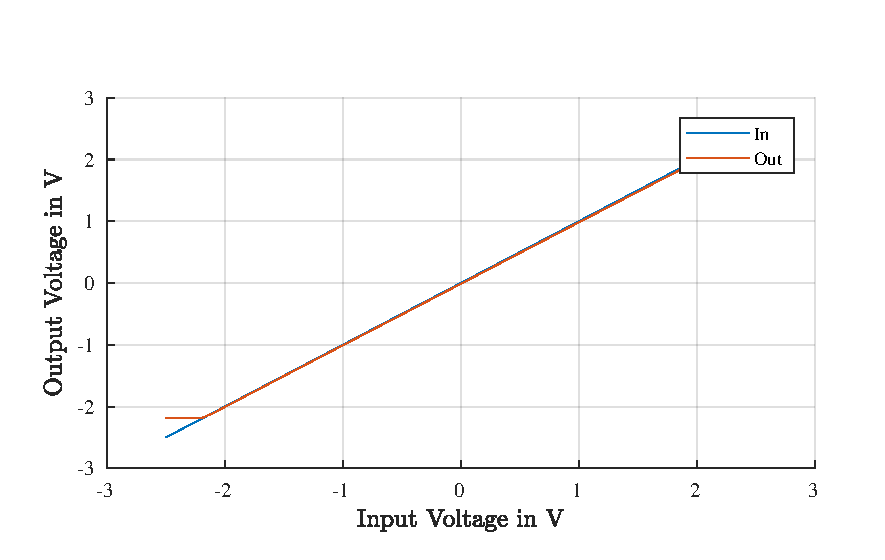
\includegraphics[scale=1]{Figures/Plots/OPAMP_ICMR.pdf}
\caption{OPAMP Plot of ICMR vs Vin}
\label{fig:OPAMP_ICMR}
\end{figure}


\begin{figure} [H]
\centering
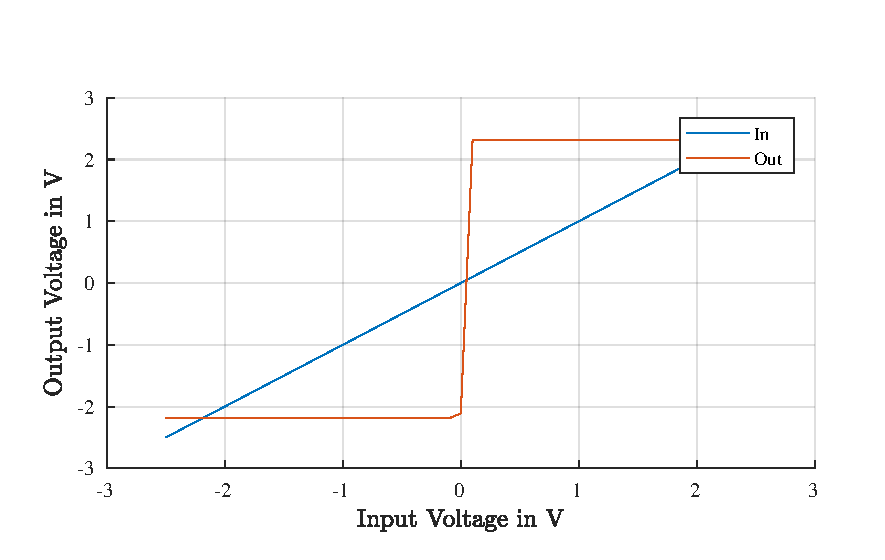
\includegraphics[scale=1]{Figures/Plots/OPAMP_OutSwing.pdf}
\caption{OPAMP Plot of Output Voltage Swing vs Vin}
\label{fig:OPAMP_Swing}
\end{figure}

\section{Corner Simulation}

\subsubsection{Process Variation - Overall System: Lowest $V_{bias}$}
\begin{figure} [H]
\centering
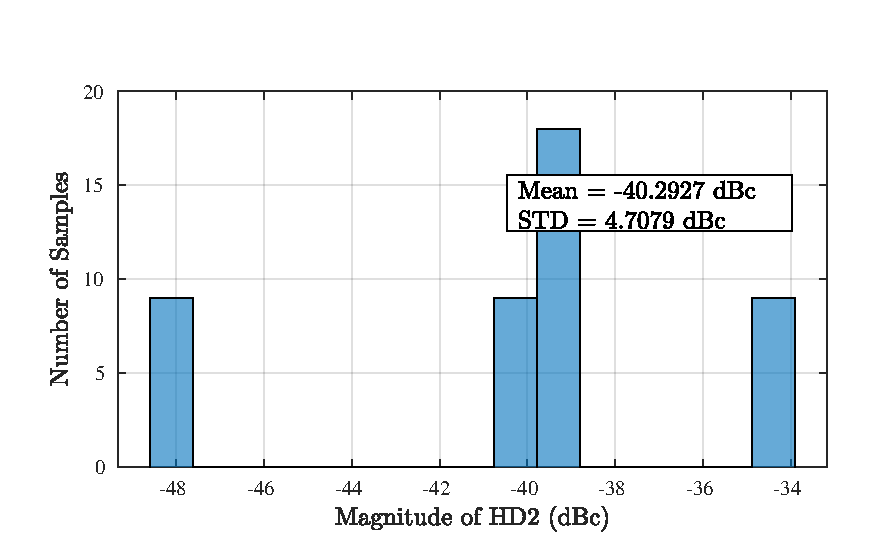
\includegraphics[scale=1]{Figures/Corners/Overall/Proc_Min/PDFs/Proc_Min_hd2.pdf}
\caption{Histogram of HD2 due to Process Variation at $V_{bias}$=150mV}
\end{figure}

\begin{figure} [H]
\centering
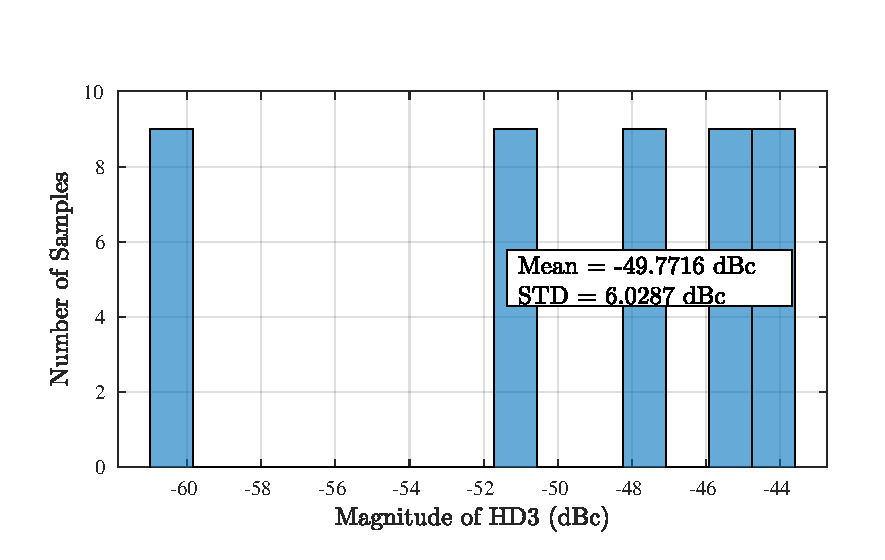
\includegraphics[scale=1]{Figures/Corners/Overall/Proc_Min/PDFs/Proc_Min_hd3.pdf}
\caption{Histogram of HD3 due to Process Variation at $V_{bias}$=150mV}
\end{figure}

\begin{figure} [H]
\centering
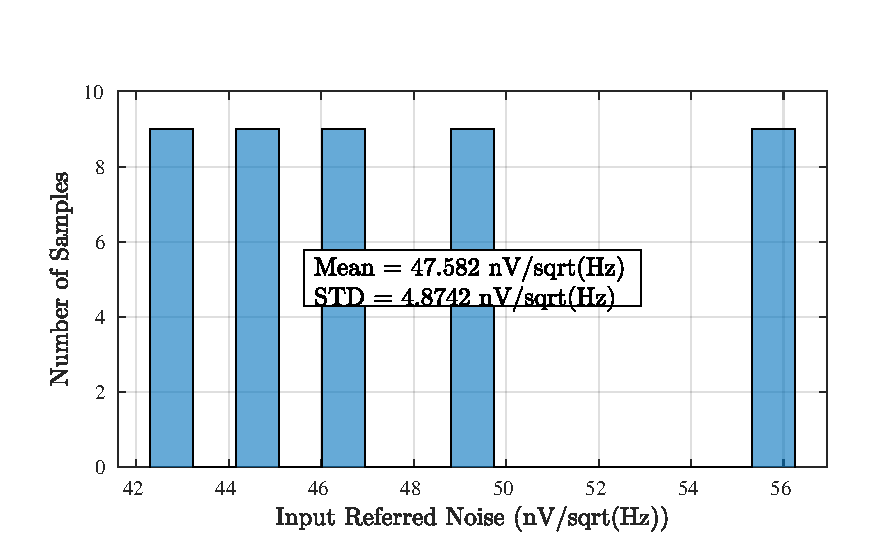
\includegraphics[scale=1]{Figures/Corners/Overall/Proc_Min/PDFs/Proc_Min_irn.pdf}
\caption{Histogram of Input Referred Noise due to Process Variation at $V_{bias}$=150mV}
\end{figure}

\begin{figure} [H]
\centering
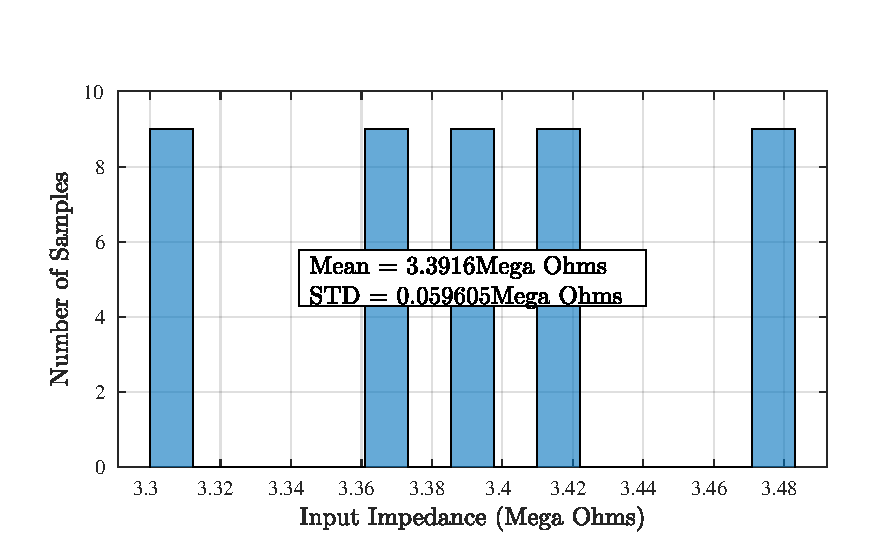
\includegraphics[scale=1]{Figures/Corners/Overall/Proc_Min/PDFs/Proc_Min_zin.pdf}
\caption{Histogram of Input Impedance due to Process Variation at $V_{bias}$=150mV}
\end{figure}

\begin{figure} [H]
\centering
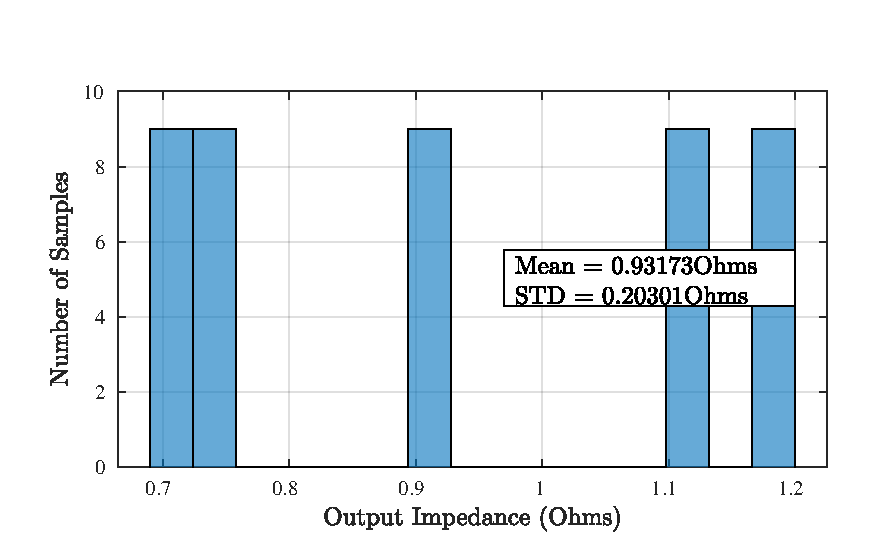
\includegraphics[scale=1]{Figures/Corners/Overall/Proc_Min/PDFs/Proc_Min_zout.pdf}
\caption{Histogram of Output Impedance due to Process Variation at $V_{bias}$=150mV}
\end{figure}

\begin{figure} [H]
\centering
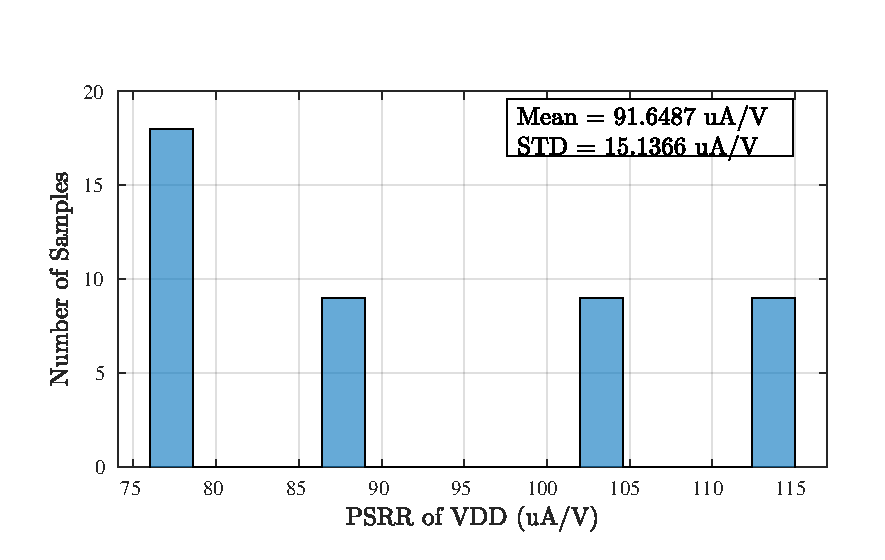
\includegraphics[scale=1]{Figures/Corners/Overall/Proc_Min/PDFs/Proc_Min_psrrp.pdf}
\caption{Histogram of PSRR($V_{DD}$) due to Process Variation at $V_{bias}$=150mV}
\end{figure}

\begin{figure} [H]
\centering
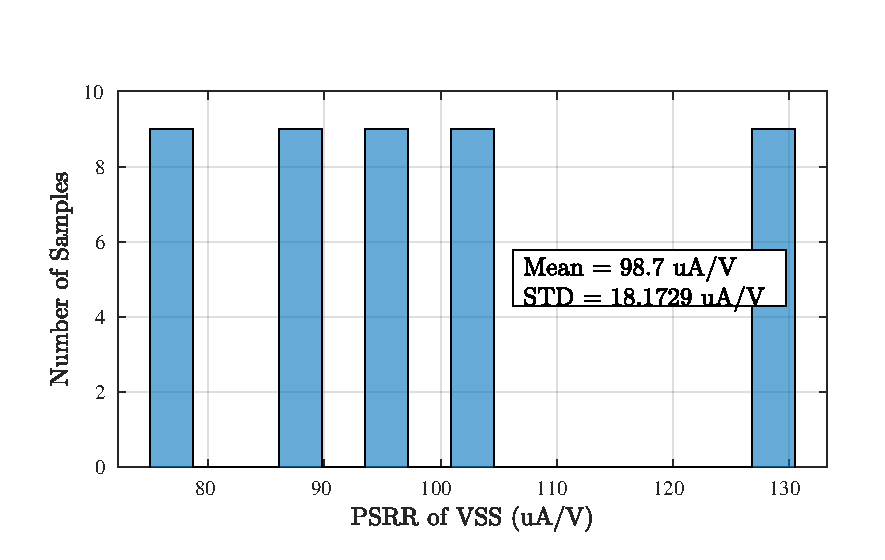
\includegraphics[scale=1]{Figures/Corners/Overall/Proc_Min/PDFs/Proc_Min_psrrn.pdf}
\caption{Histogram of PSRR($V_{SS}$) due to Process Variation at $V_{bias}$=150mV}
\end{figure}

\subsubsection{Process Variation - Overall System: Middle $V_{bias}$}
\begin{figure} [H]
\centering
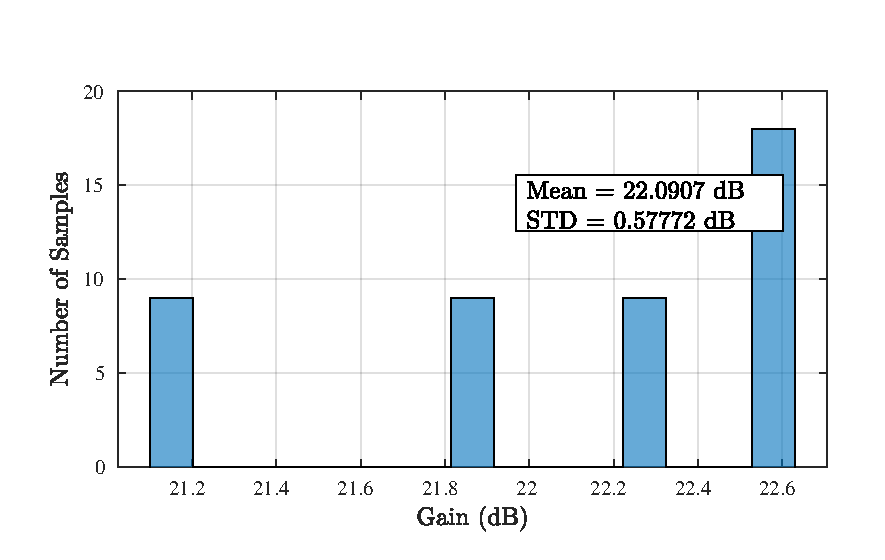
\includegraphics[scale=1]{Figures/Corners/Overall/Proc_Mid/PDFs/Proc_Mid_gain.pdf}
\caption{Histogram of System Gain due to Process Variation at $V_{bias}$=400mV}
\end{figure}

\begin{figure} [H]
\centering
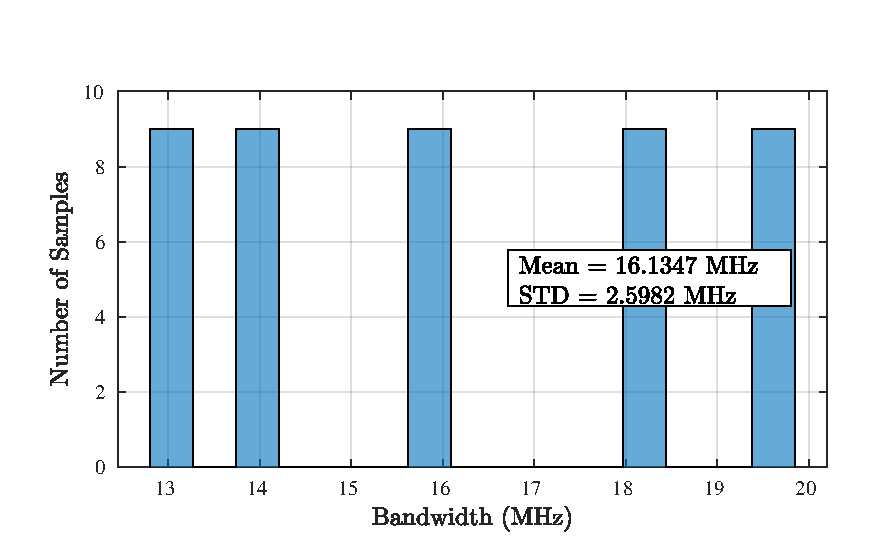
\includegraphics[scale=1]{Figures/Corners/Overall/Proc_Mid/PDFs/Proc_Mid_bw.pdf}
\caption{Histogram of System Bandwidth due to Process Variation at $V_{bias}$=400mV}
\end{figure}

\begin{figure} [H]
\centering
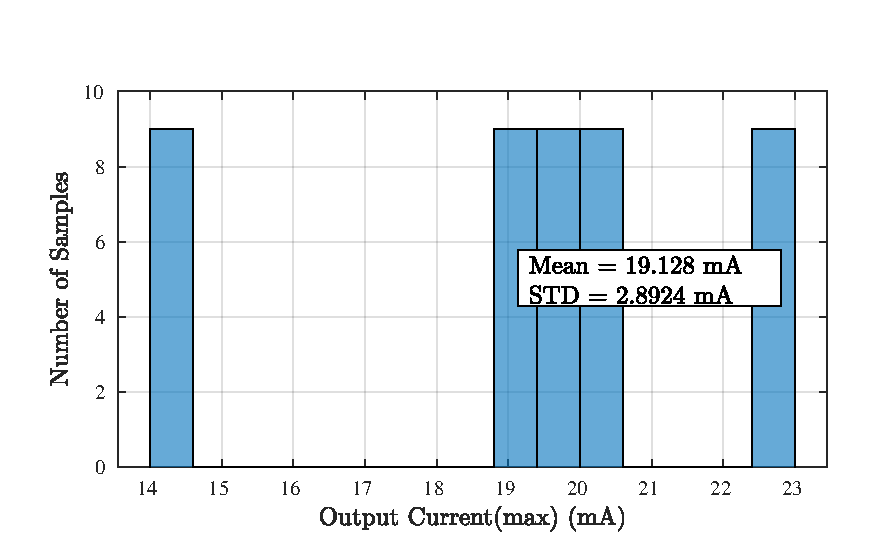
\includegraphics[scale=1]{Figures/Corners/Overall/Proc_Mid/PDFs/Proc_Mid_imax.pdf}
\caption{Histogram of Maximum Output Current due to Process Variation at $V_{bias}$=400mV}
\end{figure}

\begin{figure} [H]
\centering
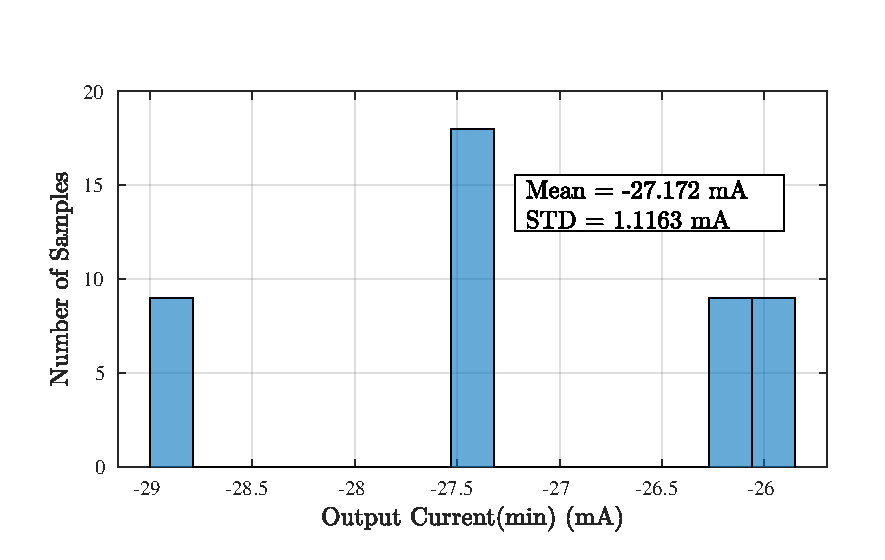
\includegraphics[scale=1]{Figures/Corners/Overall/Proc_Mid/PDFs/Proc_Mid_imin.pdf}
\caption{Histogram of Minimum Output Current due to Process Variation at $V_{bias}$=400mV}
\end{figure}

\begin{figure} [H]
\centering
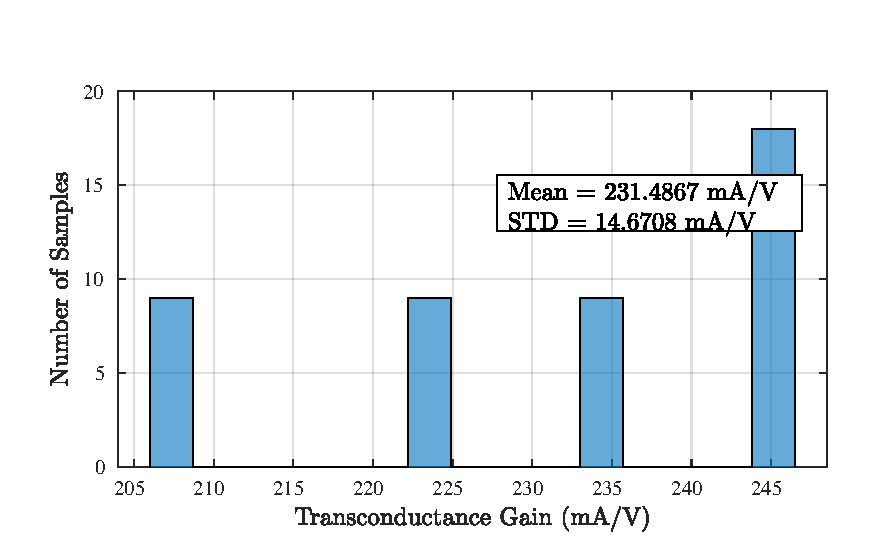
\includegraphics[scale=1]{Figures/Corners/Overall/Proc_Mid/PDFs/Proc_Mid_gm.pdf}
\caption{Histogram of Transconductance due to Process Variation at $V_{bias}$=400mV}
\end{figure}

\begin{figure} [H]
\centering
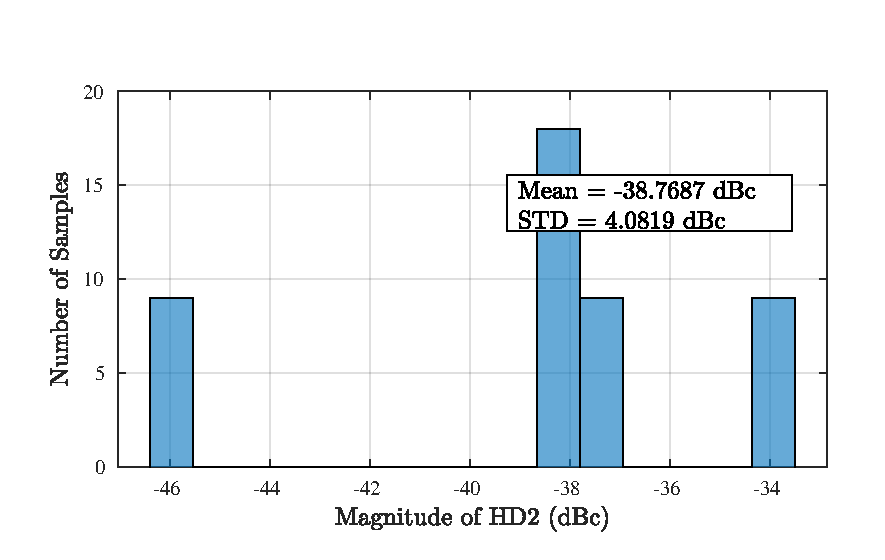
\includegraphics[scale=1]{Figures/Corners/Overall/Proc_Mid/PDFs/Proc_Mid_hd2.pdf}
\caption{Histogram of HD2 due to Process Variation at $V_{bias}$=400mV}
\end{figure}

\begin{figure} [H]
\centering
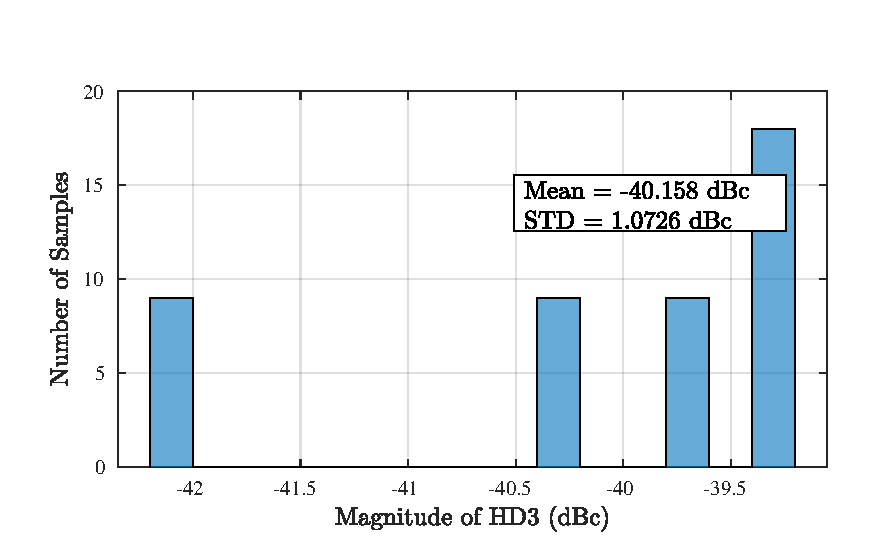
\includegraphics[scale=1]{Figures/Corners/Overall/Proc_Mid/PDFs/Proc_Mid_hd3.pdf}
\caption{Histogram of HD3 due to Process Variation at $V_{bias}$=400mV}
\end{figure}

\begin{figure} [H]
\centering
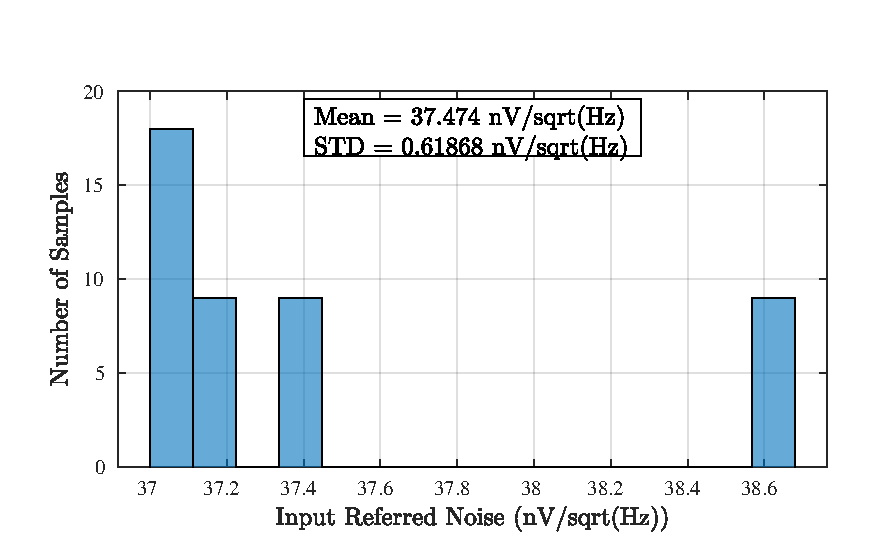
\includegraphics[scale=1]{Figures/Corners/Overall/Proc_Mid/PDFs/Proc_Mid_irn.pdf}
\caption{Histogram of Input Referred Noise due to Process Variation at $V_{bias}$=400mV}
\end{figure}

\begin{figure} [H]
\centering
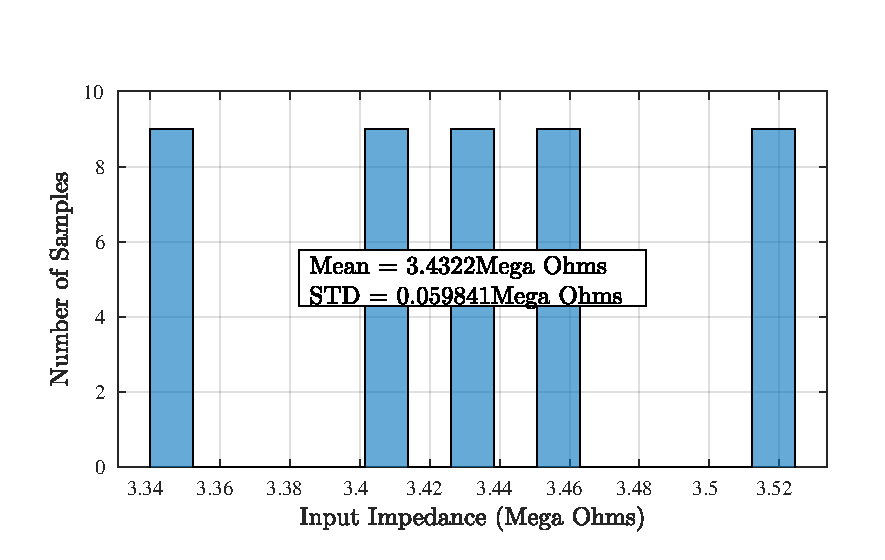
\includegraphics[scale=1]{Figures/Corners/Overall/Proc_Mid/PDFs/Proc_Mid_zin.pdf}
\caption{Histogram of Input Impedance due to Process Variation at $V_{bias}$=400mV}
\end{figure}

\begin{figure} [H]
\centering
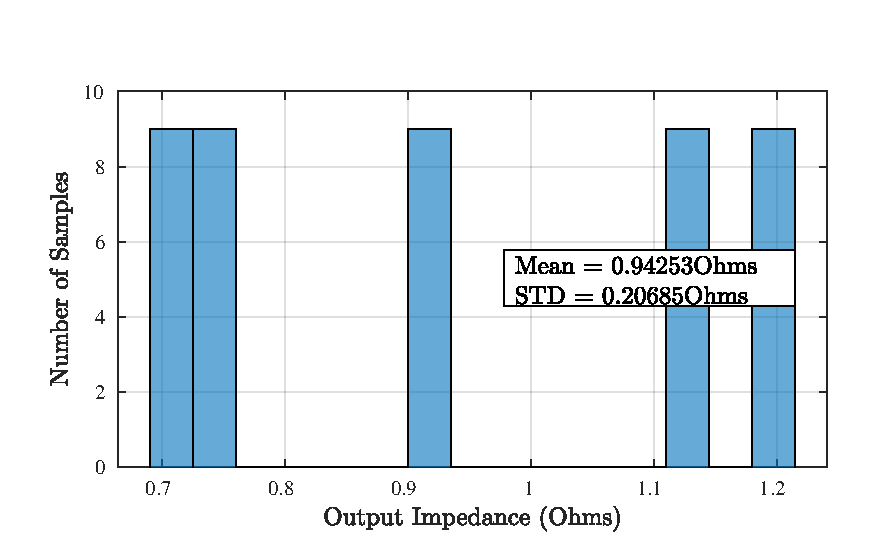
\includegraphics[scale=1]{Figures/Corners/Overall/Proc_Mid/PDFs/Proc_Mid_zout.pdf}
\caption{Histogram of Output Impedance due to Process Variation at $V_{bias}$=400mV}
\end{figure}

\begin{figure} [H]
\centering
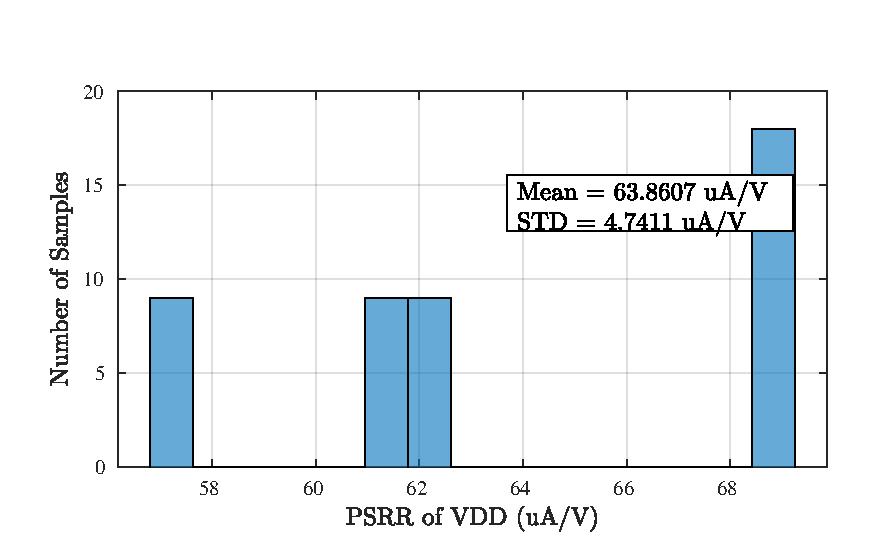
\includegraphics[scale=1]{Figures/Corners/Overall/Proc_Mid/PDFs/Proc_Mid_psrrp.pdf}
\caption{Histogram of PSRR($V_{DD}$) due to Process Variation at $V_{bias}$=400mV}
\end{figure}

\begin{figure} [H]
\centering
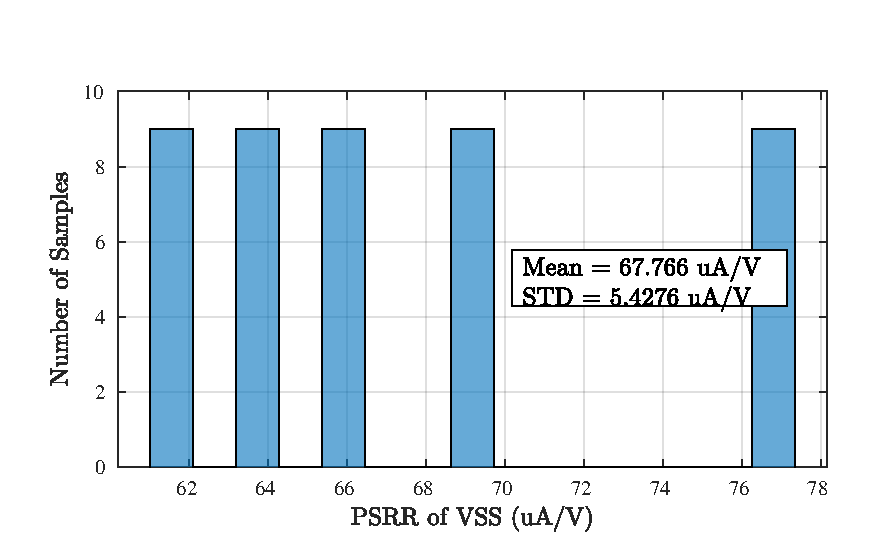
\includegraphics[scale=1]{Figures/Corners/Overall/Proc_Mid/PDFs/Proc_Mid_psrrn.pdf}
\caption{Histogram of PSRR($V_{SS}$) due to Process Variation at $V_{bias}$=400mV}
\end{figure}

\subsubsection{Process Variation - Overall System: Highest $V_{bias}$}

\begin{figure} [H]
\centering
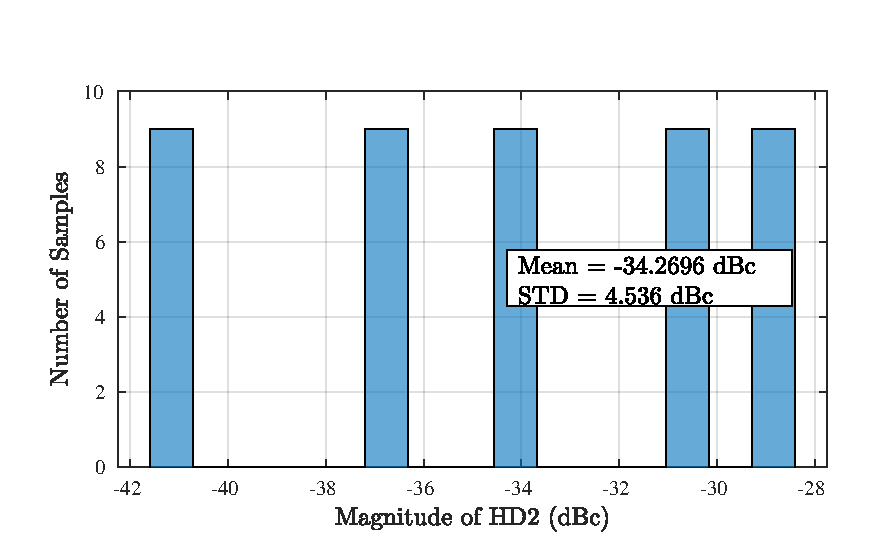
\includegraphics[scale=1]{Figures/Corners/Overall/Proc_Max/PDFs/Proc_Max_hd2.pdf}
\caption{Histogram of HD2 due to Process Variation at $V_{bias}$=700mV}
\end{figure}

\begin{figure} [H]
\centering
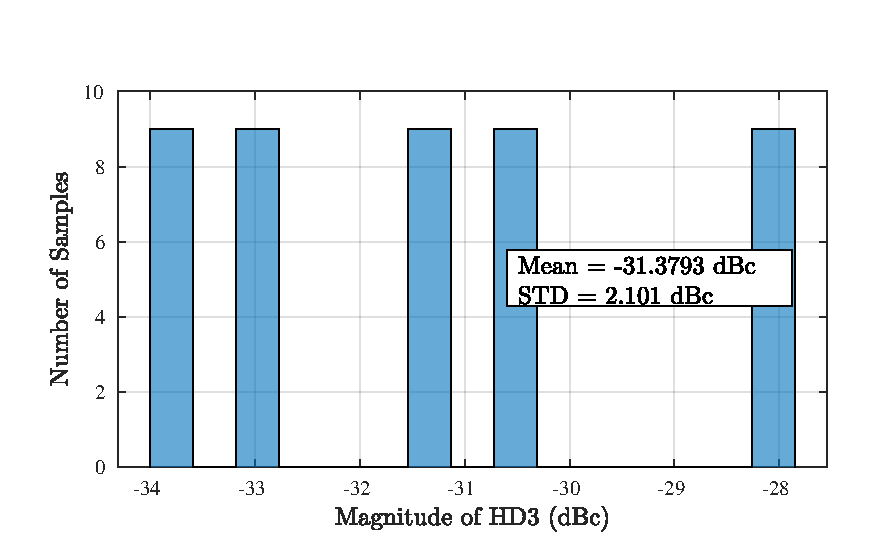
\includegraphics[scale=1]{Figures/Corners/Overall/Proc_Max/PDFs/Proc_Max_hd3.pdf}
\caption{Histogram of HD3 due to Process Variation at $V_{bias}$=700mV}
\end{figure}

\begin{figure} [H]
\centering
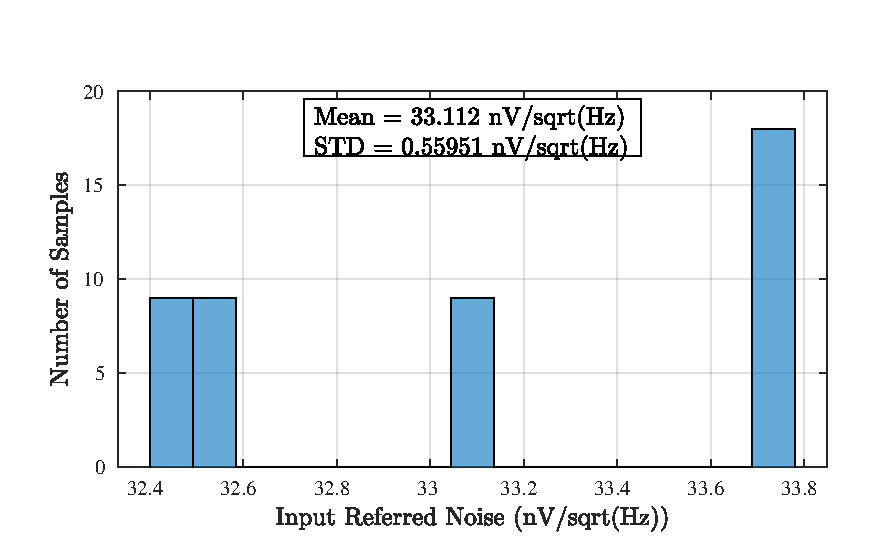
\includegraphics[scale=1]{Figures/Corners/Overall/Proc_Max/PDFs/Proc_Max_irn.pdf}
\caption{Histogram of Input Referred Noise due to Process Variation at $V_{bias}$=400mV}
\end{figure}

\begin{figure} [H]
\centering
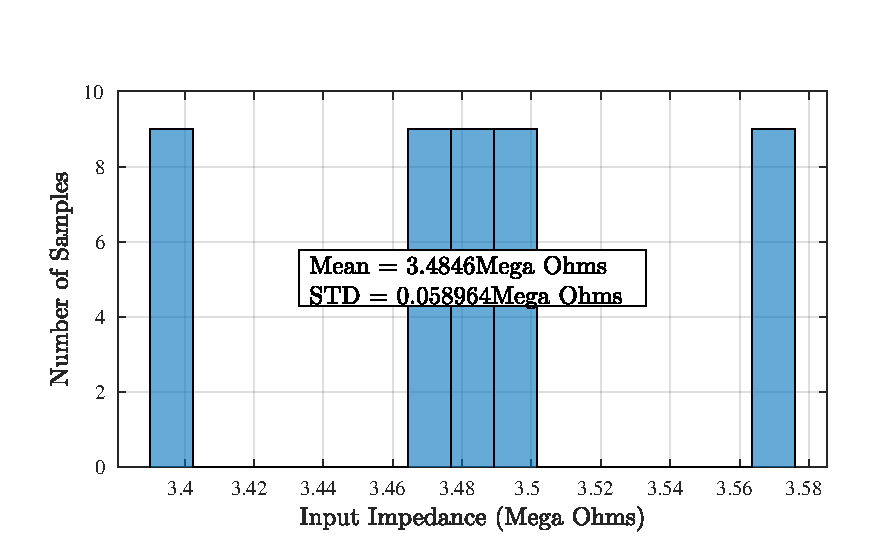
\includegraphics[scale=1]{Figures/Corners/Overall/Proc_Max/PDFs/Proc_Max_zin.pdf}
\caption{Histogram of Input Impedance due to Process Variation at $V_{bias}$=700mV}
\end{figure}

\begin{figure} [H]
\centering
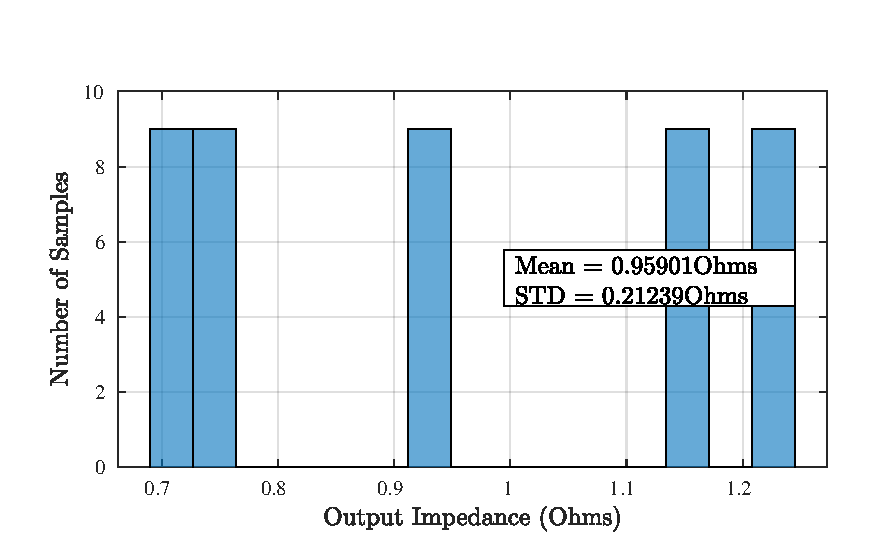
\includegraphics[scale=1]{Figures/Corners/Overall/Proc_Max/PDFs/Proc_Max_zout.pdf}
\caption{Histogram of Output Impedance due to Process Variation at $V_{bias}$=700mV}
\end{figure}

\begin{figure} [H]
\centering
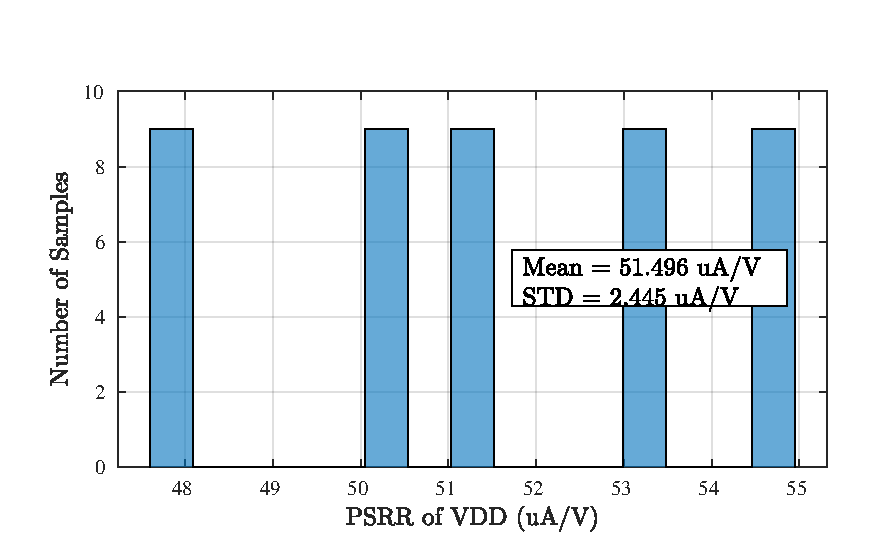
\includegraphics[scale=1]{Figures/Corners/Overall/Proc_Max/PDFs/Proc_Max_psrrp.pdf}
\caption{Histogram of PSRR($V_{DD}$) due to Process Variation at $V_{bias}$=700mV}
\end{figure}

\begin{figure} [H]
\centering
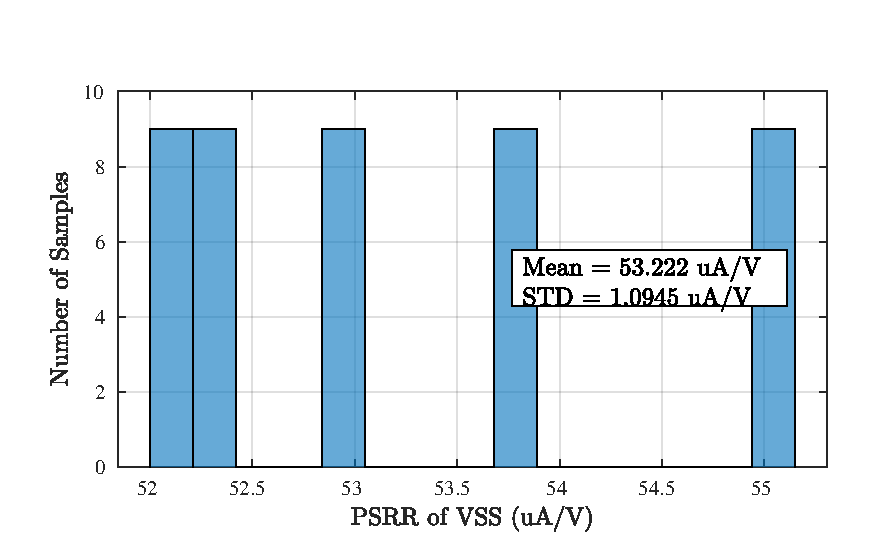
\includegraphics[scale=1]{Figures/Corners/Overall/Proc_Max/PDFs/Proc_Max_psrrn.pdf}
\caption{Histogram of PSRR($V_{SS}$) due to Process Variation at $V_{bias}$=700mV}
\end{figure}


\subsubsection{Process and Supply Variation - Overeall System: Lowest $V_{bias}$}
\begin{figure} [H]
\centering
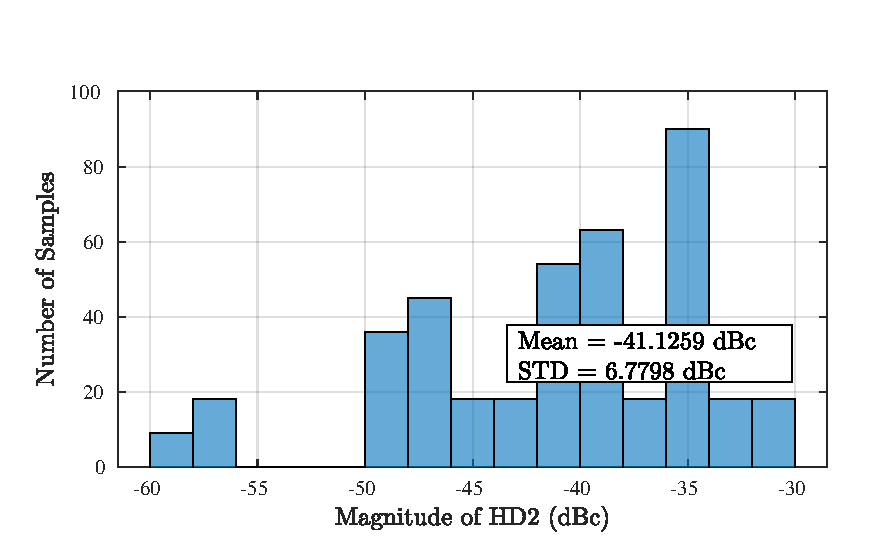
\includegraphics[scale=1]{Figures/Corners/Overall/PV_Min/PDFs/PV_Min_hd2.pdf}
\caption{Histogram of HD2 due to Process and Supply Variation at $V_{bias}$=150mV}
\end{figure}

\begin{figure} [H]
\centering
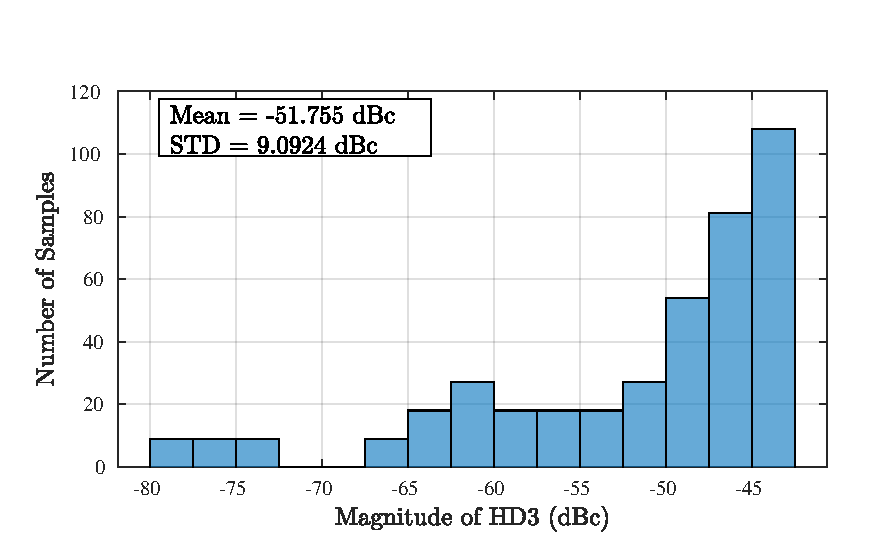
\includegraphics[scale=1]{Figures/Corners/Overall/PV_Min/PDFs/PV_Min_hd3.pdf}
\caption{Histogram of HD3 due to Process and Supply Variation at $V_{bias}$=150mV}
\end{figure}

\begin{figure} [H]
\centering
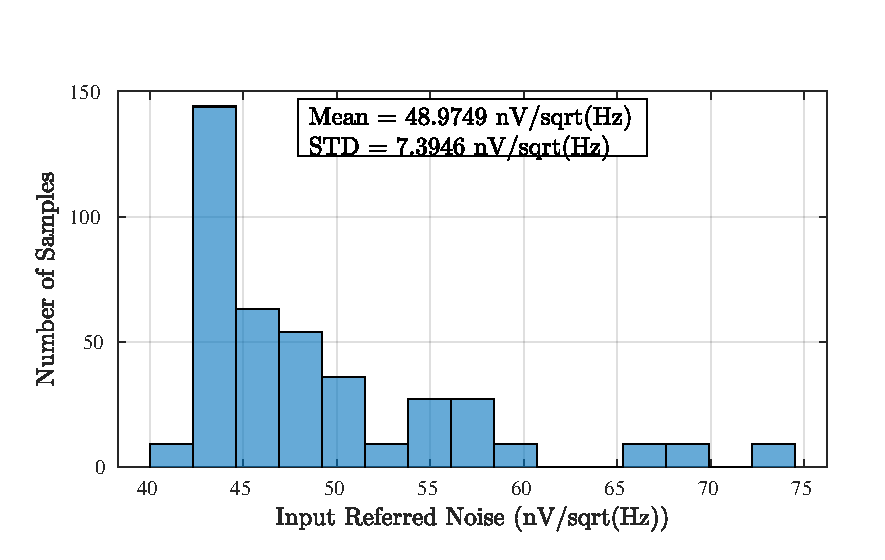
\includegraphics[scale=1]{Figures/Corners/Overall/PV_Min/PDFs/PV_Min_irn.pdf}
\caption{Histogram of Input Referred Noise due to Process and Supply Variation at $V_{bias}$=150mV}
\end{figure}

\begin{figure} [H]
\centering
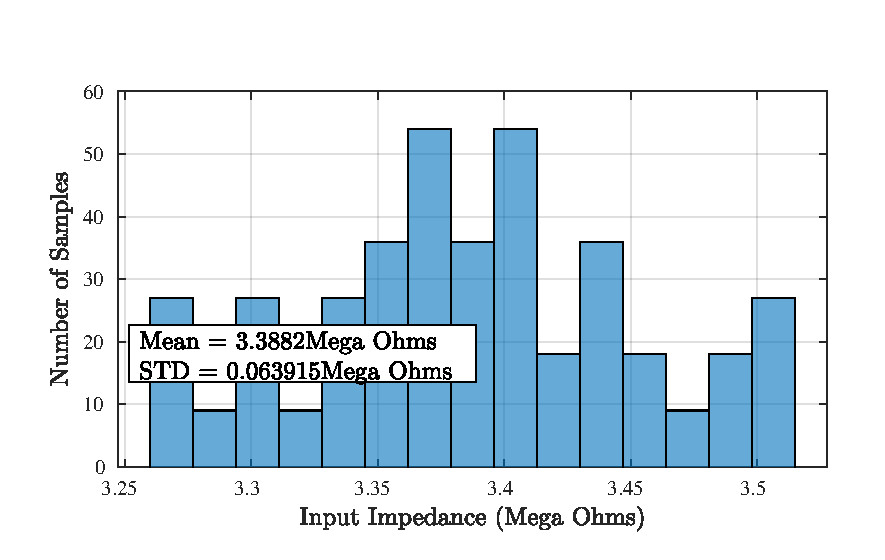
\includegraphics[scale=1]{Figures/Corners/Overall/PV_Min/PDFs/PV_Min_zin.pdf}
\caption{Histogram of Input Impedance due to Process and Supply Variation at $V_{bias}$=150mV}
\end{figure}

\begin{figure} [H]
\centering
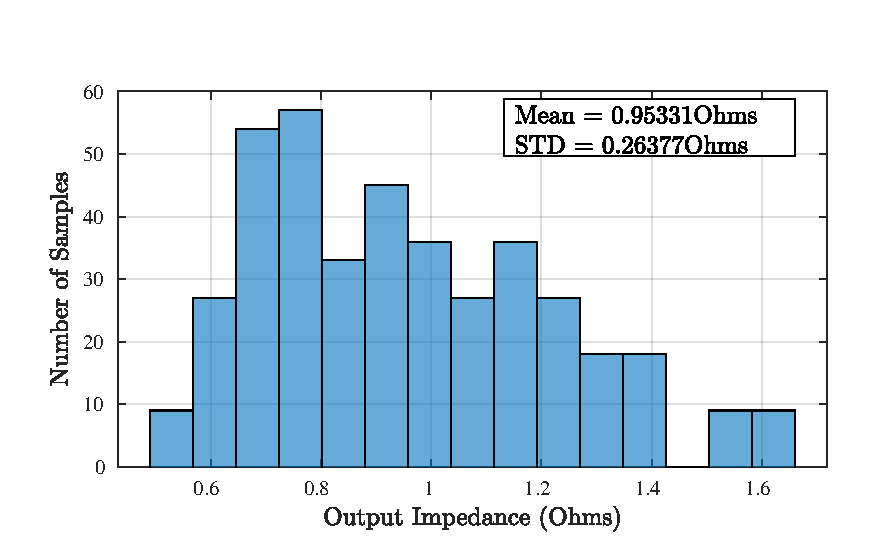
\includegraphics[scale=1]{Figures/Corners/Overall/PV_Min/PDFs/PV_Min_zout.pdf}
\caption{Histogram of Output Impedance due to Process and Supply Variation at $V_{bias}$=150mV}
\end{figure}

\begin{figure} [H]
\centering
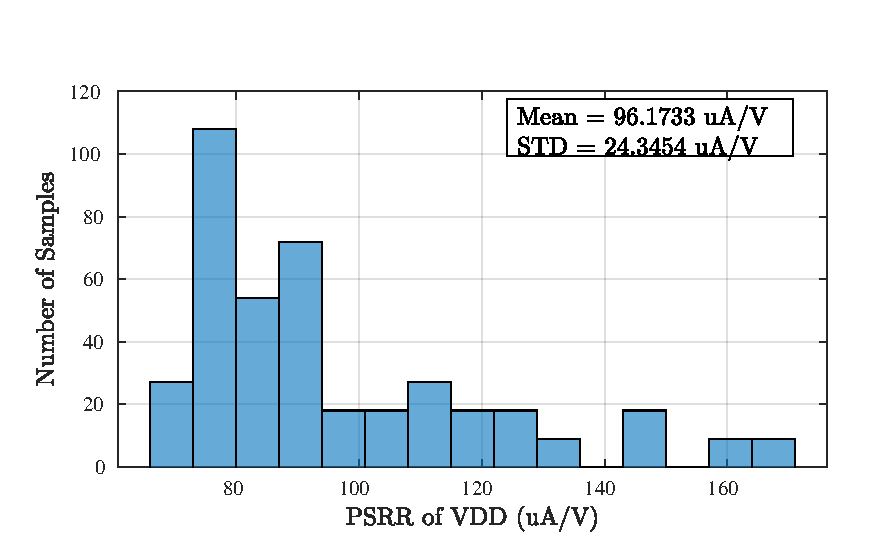
\includegraphics[scale=1]{Figures/Corners/Overall/PV_Min/PDFs/PV_Min_psrrp.pdf}
\caption{Histogram of PSRR($V_{DD}$) due to Process and SUpply Variation at $V_{bias}$=150mV}
\end{figure}

\begin{figure} [H]
\centering
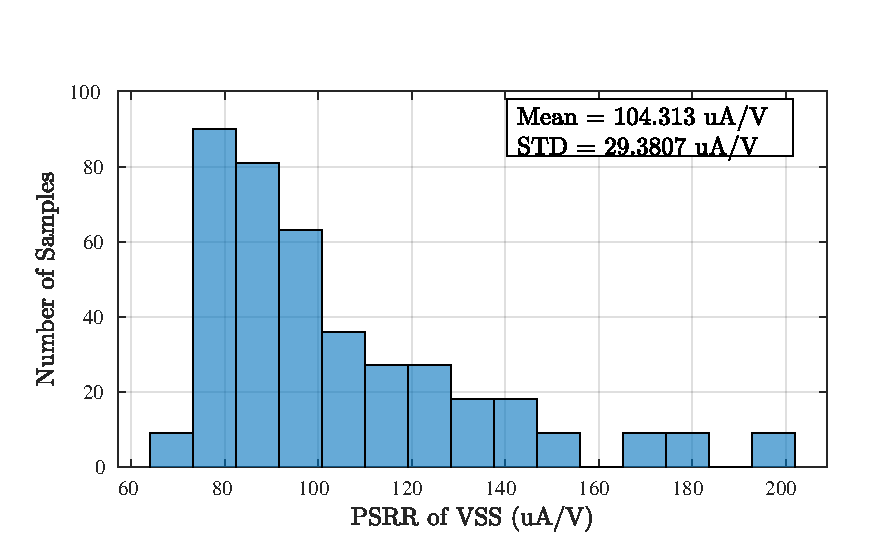
\includegraphics[scale=1]{Figures/Corners/Overall/PV_Min/PDFs/PV_Min_psrrn.pdf}
\caption{Histogram of PSRR($V_{SS}$) due to Process and SUpply Variation at $V_{bias}$=150mV}
\end{figure}

\subsubsection{Process and Supply Variation - Overeall System: Middle $V_{bias}$}

\begin{figure} [H]
\centering
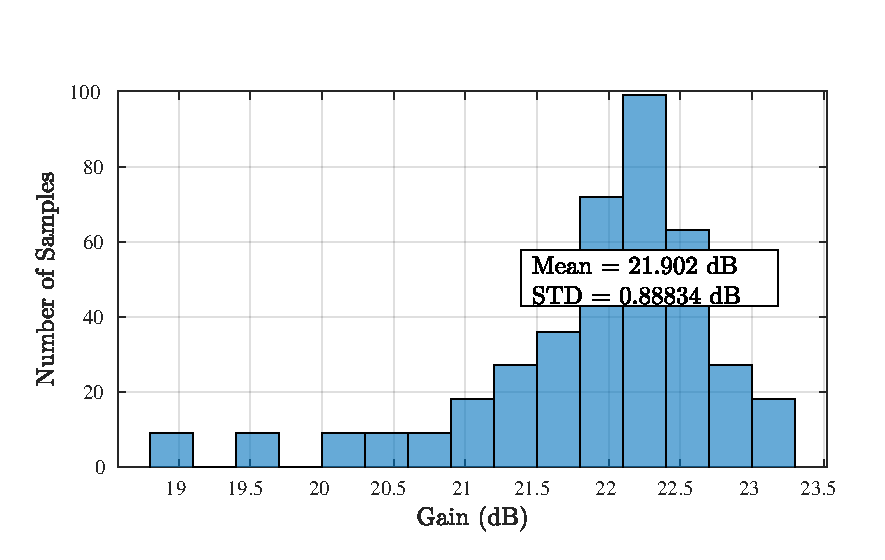
\includegraphics[scale=1]{Figures/Corners/Overall/PV_Mid/PDFs/PV_Mid_gain.pdf}
\caption{Histogram of System Gain due to Process and Supply Variation at $V_{bias}$=400mV}
\end{figure}

\begin{figure} [H]
\centering
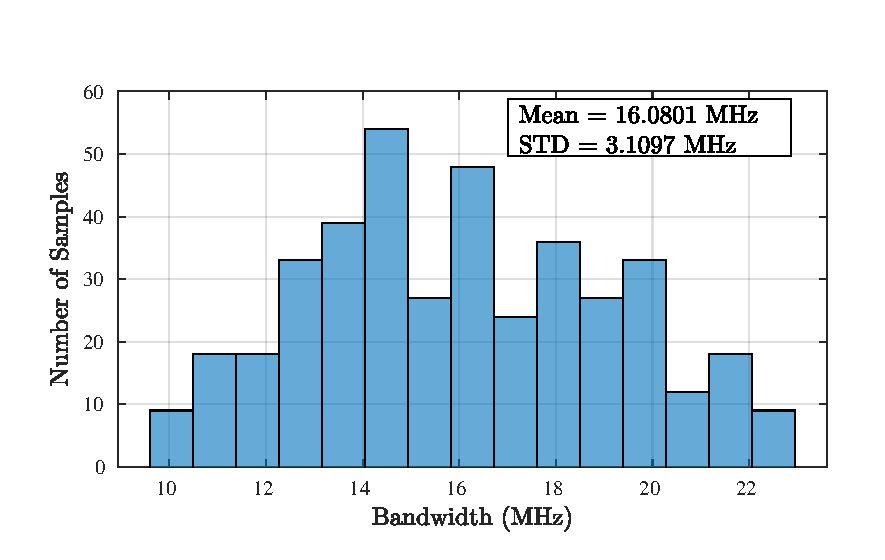
\includegraphics[scale=1]{Figures/Corners/Overall/PV_Mid/PDFs/PV_Mid_bw.pdf}
\caption{Histogram of System Bandwidth due to Process and Supply Variation at $V_{bias}$=400mV}
\end{figure}

\begin{figure} [H]
\centering
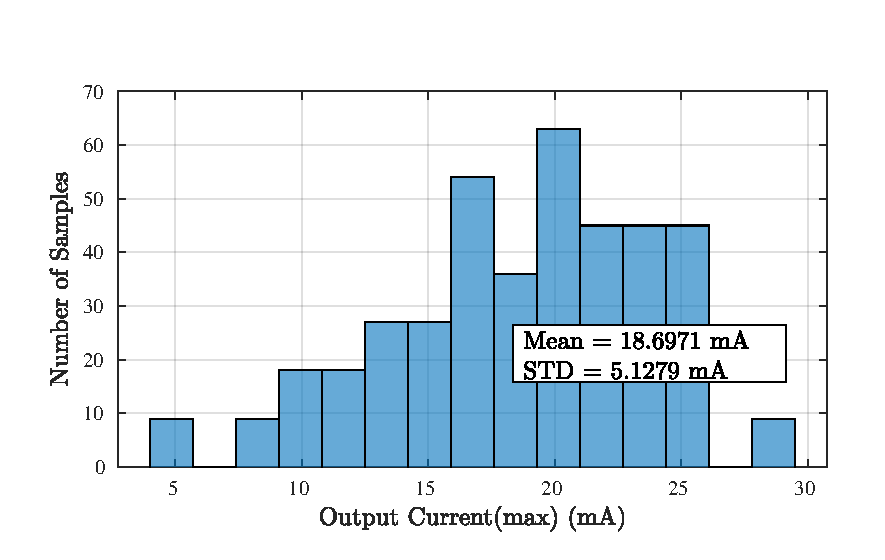
\includegraphics[scale=1]{Figures/Corners/Overall/PV_Mid/PDFs/PV_Mid_imax.pdf}
\caption{Histogram of Maximum Output Current due to Process and Supply Variation at $V_{bias}$=400mV}
\end{figure}

\begin{figure} [H]
\centering
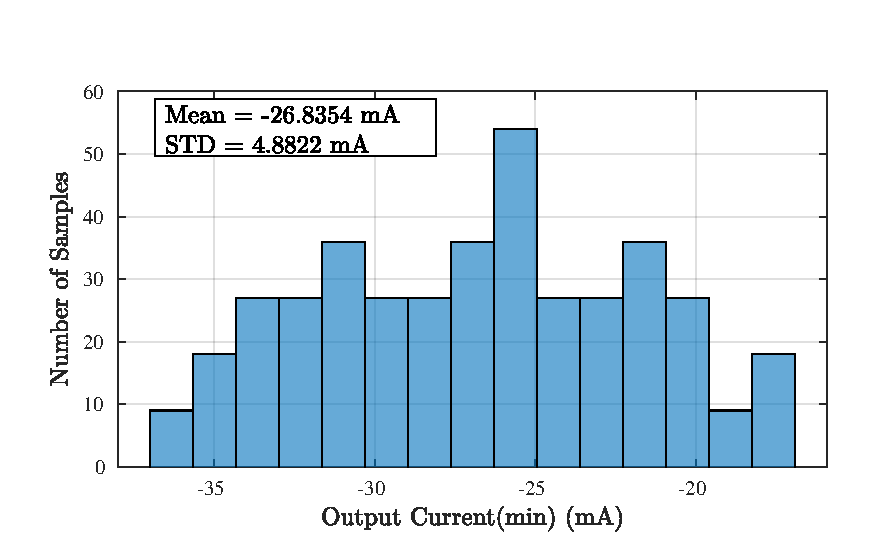
\includegraphics[scale=1]{Figures/Corners/Overall/PV_Mid/PDFs/PV_Mid_imin.pdf}
\caption{Histogram of Minimum Output Current due to Process and Supply Variation at $V_{bias}$=400mV}
\end{figure}

\begin{figure} [H]
\centering
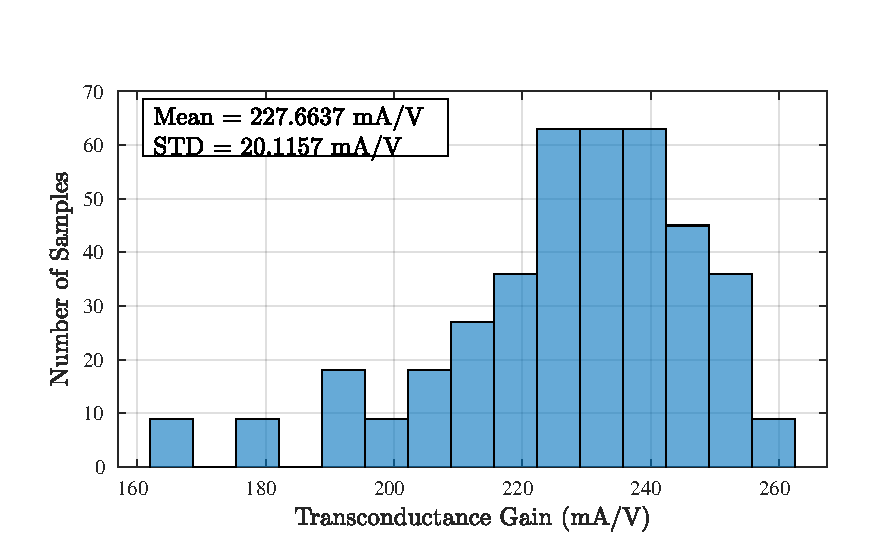
\includegraphics[scale=1]{Figures/Corners/Overall/PV_Mid/PDFs/PV_Mid_gm.pdf}
\caption{Histogram of Transconductance due to Process and Supply Variation at $V_{bias}$=400mV}
\end{figure}

\begin{figure} [H]
\centering
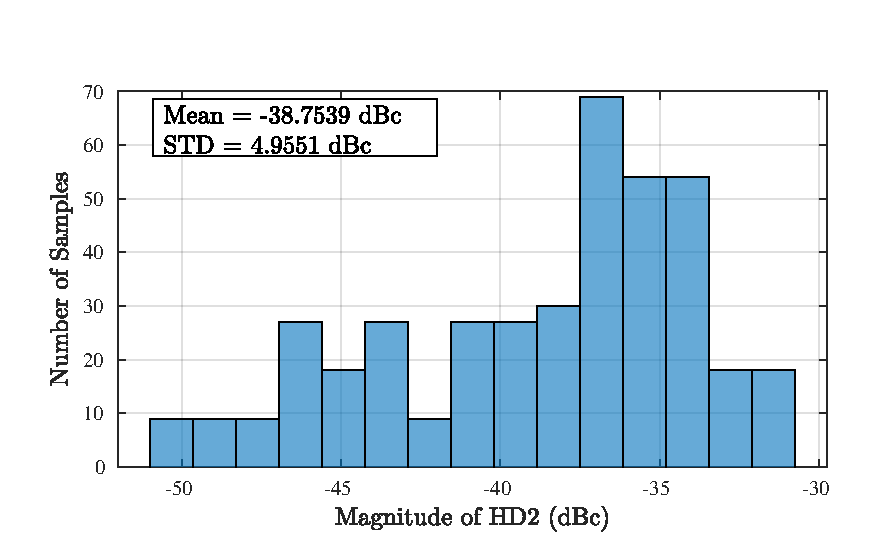
\includegraphics[scale=1]{Figures/Corners/Overall/PV_Mid/PDFs/PV_Mid_hd2.pdf}
\caption{Histogram of HD2 due to Process and Supply Variation at $V_{bias}$=400mV}
\end{figure}

\begin{figure} [H]
\centering
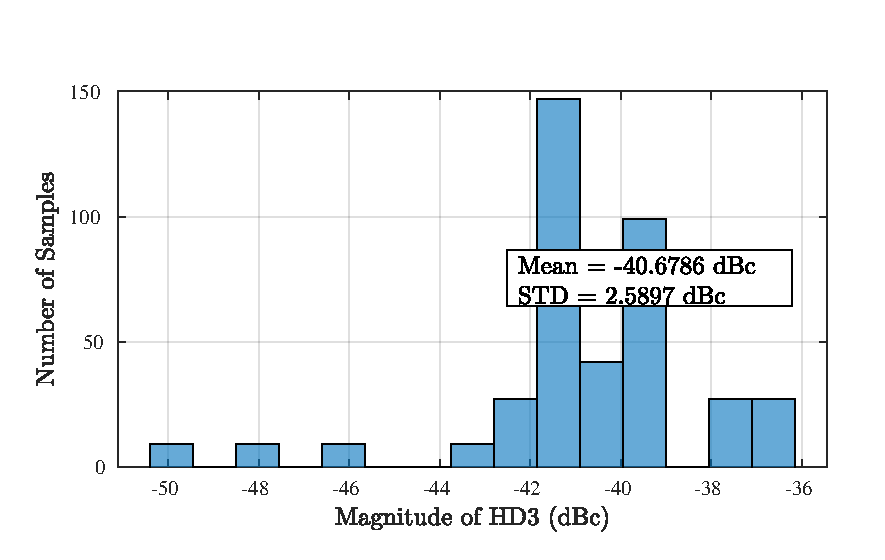
\includegraphics[scale=1]{Figures/Corners/Overall/PV_Mid/PDFs/PV_Mid_hd3.pdf}
\caption{Histogram of HD3 due to Process and Supply Variation at $V_{bias}$=400mV}
\end{figure}

\begin{figure} [H]
\centering
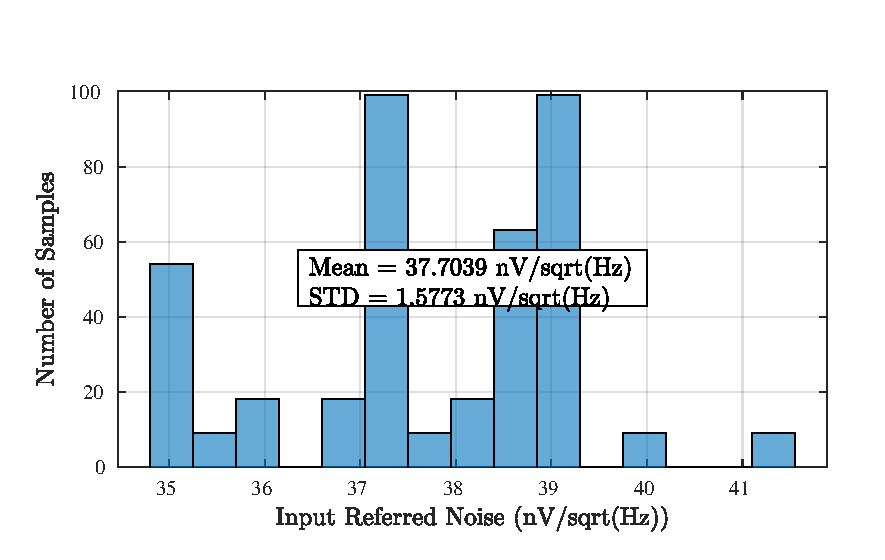
\includegraphics[scale=1]{Figures/Corners/Overall/PV_Mid/PDFs/PV_Mid_irn.pdf}
\caption{Histogram of Input Referred Noise due to Process and Supply Variation at $V_{bias}$=400mV}
\end{figure}

\begin{figure} [H]
\centering
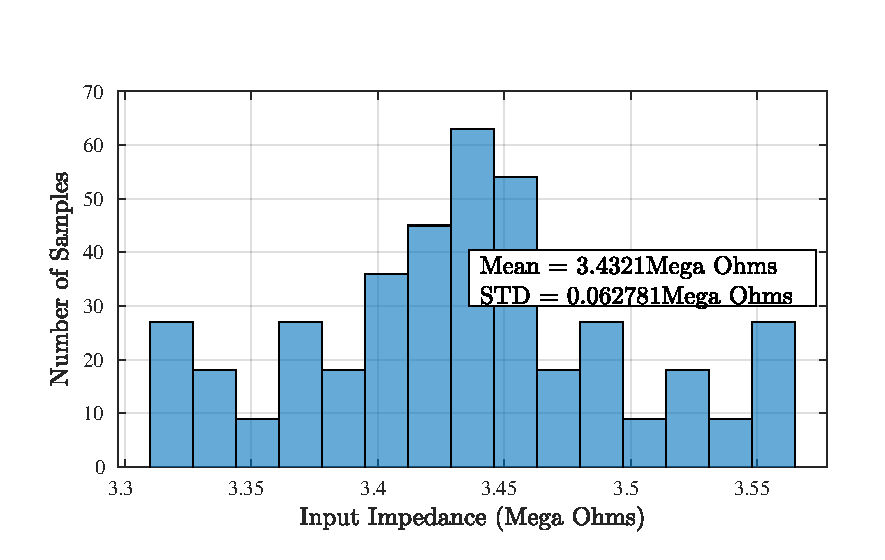
\includegraphics[scale=1]{Figures/Corners/Overall/PV_Mid/PDFs/PV_Mid_zin.pdf}
\caption{Histogram of Input Impedance due to Process and Supply Variation at $V_{bias}$=400mV}
\end{figure}

\begin{figure} [H]
\centering
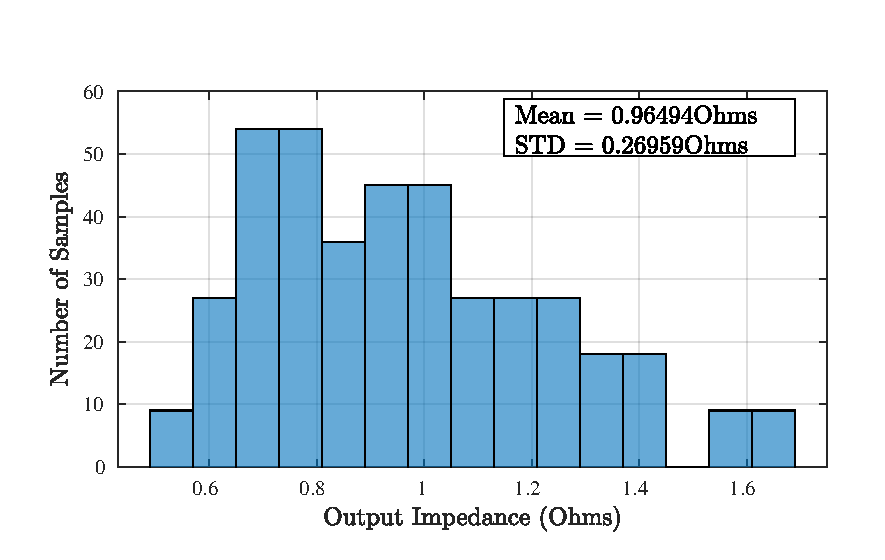
\includegraphics[scale=1]{Figures/Corners/Overall/PV_Mid/PDFs/PV_Mid_zout.pdf}
\caption{Histogram of Output Impedance due to Process and Supply Variation at $V_{bias}$=400mV}
\end{figure}

\begin{figure} [H]
\centering
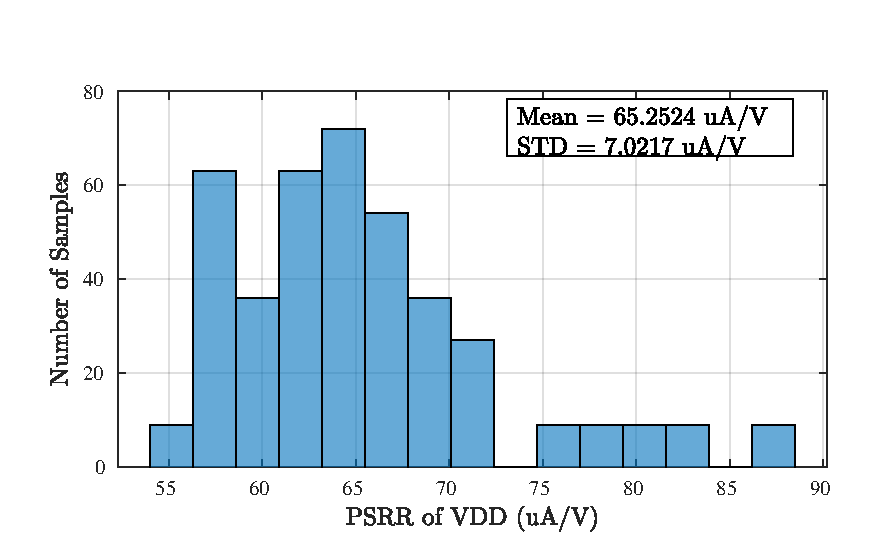
\includegraphics[scale=1]{Figures/Corners/Overall/PV_Mid/PDFs/PV_Mid_psrrp.pdf}
\caption{Histogram of PSRR($V_{DD}$) due to Process and Supply Variation at $V_{bias}$=400mV}
\end{figure}

\begin{figure} [H]
\centering
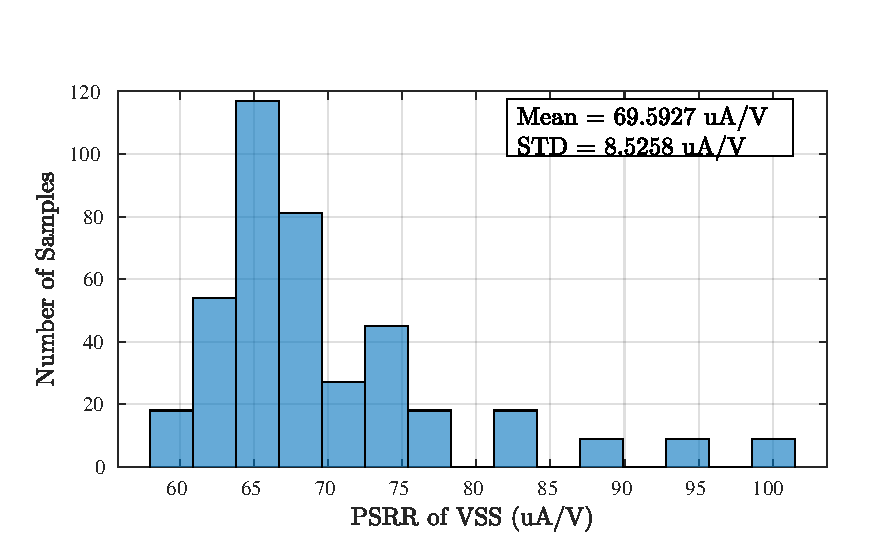
\includegraphics[scale=1]{Figures/Corners/Overall/PV_Mid/PDFs/PV_Mid_psrrn.pdf}
\caption{Histogram of PSRR($V_{SS}$) due to Process and Supply Variation at $V_{bias}$=400mV}
\end{figure}

\subsubsection{Process and Supply Variation - Overeall System: Highest $V_{bias}$}
\begin{figure} [H]
\centering
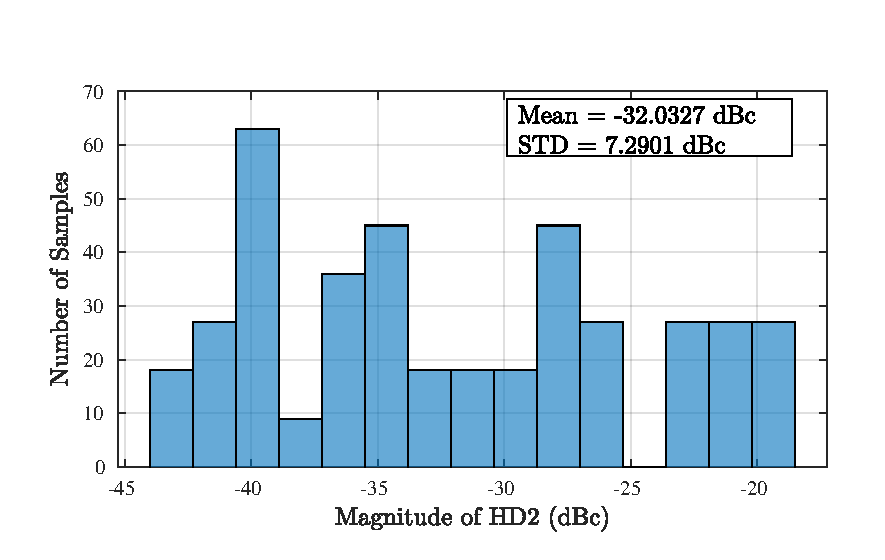
\includegraphics[scale=1]{Figures/Corners/Overall/PV_Max/PDFs/PV_Max_hd2.pdf}
\caption{Histogram of HD2 due to Process and Supply Variation at $V_{bias}$=700mV}
\end{figure}

\begin{figure} [H]
\centering
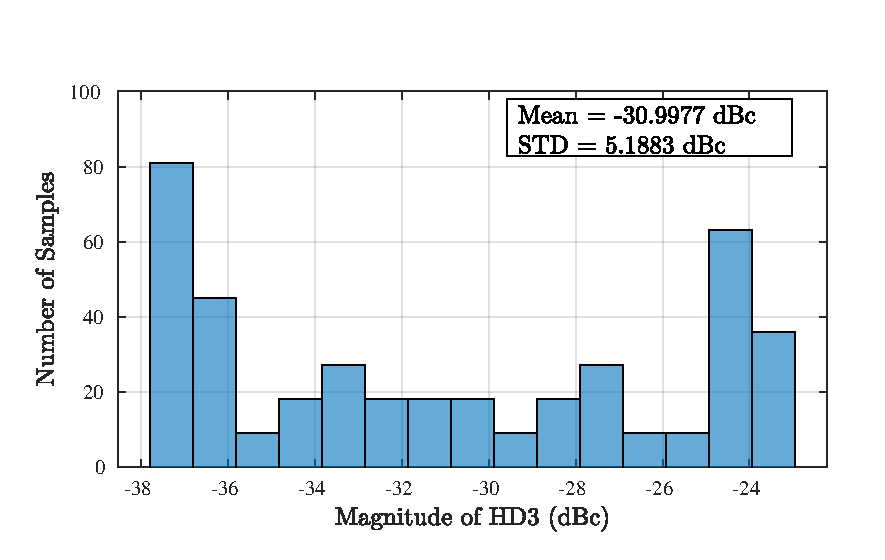
\includegraphics[scale=1]{Figures/Corners/Overall/PV_Max/PDFs/PV_Max_hd3.pdf}
\caption{Histogram of HD3 due to Process and Supply Variation at $V_{bias}$=700mV}
\end{figure}

\begin{figure} [H]
\centering
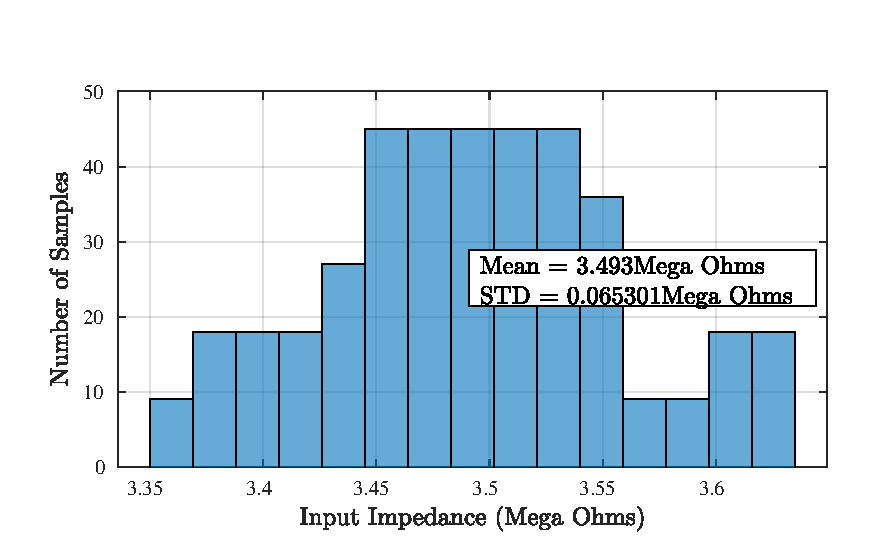
\includegraphics[scale=1]{Figures/Corners/Overall/PV_Max/PDFs/PV_Max_zin.pdf}
\caption{Histogram of Input Impedance due to Process and Supply Variation at $V_{bias}$=700mV}
\end{figure}

\begin{figure} [H]
\centering
\includegraphics[scale=1]{Figures/Corners/Overall/PV_Max/PDFs/PV_Max_zout.pdf}
\caption{Histogram of Output Impedance due to Process and Supply Variation at $V_{bias}$=700mV}
\end{figure}

\begin{figure} [H]
\centering
\includegraphics[scale=1]{Figures/Corners/Overall/PV_Max/PDFs/PV_Max_psrrp.pdf}
\caption{Histogram of PSRR($V_{DD}$) due to Process and Supply Variation at $V_{bias}$=700mV}
\end{figure}

\begin{figure} [H]
\centering
\includegraphics[scale=1]{Figures/Corners/Overall/PV_Max/PDFs/PV_Max_psrrn.pdf}
\caption{Histogram of PSRR($V_{SS}$) due to Process and Supply Variation at $V_{bias}$=700mV}
\end{figure}

\subsubsection{PVT: Overall - Middle $V_{bias}$}

\begin{figure} [H]
\centering
\includegraphics[scale=1]{Figures/Corners/Overall/PVT_Mid/PDFs/PVT_Mid_gain.pdf}
\caption{Histogram of System Gain due to PVT Variation at $V_{bias}$=400mV}
\end{figure}

\begin{figure} [H]
\centering
\includegraphics[scale=1]{Figures/Corners/Overall/PVT_Mid/PDFs/PVT_Mid_bw.pdf}
\caption{Histogram of System Bandwidth due to PVT Variation at $V_{bias}$=400mV}
\end{figure}

\begin{figure} [H]
\centering
\includegraphics[scale=1]{Figures/Corners/Overall/PVT_Mid/PDFs/PVT_Mid_imax.pdf}
\caption{Histogram of Maximum Output Current due to PVT Variation at $V_{bias}$=400mV}
\end{figure}

\begin{figure} [H]
\centering
\includegraphics[scale=1]{Figures/Corners/Overall/PVT_Mid/PDFs/PVT_Mid_imin.pdf}
\caption{Histogram of Minimum Output Current due to PVT Variation at $V_{bias}$=400mV}
\end{figure}

\begin{figure} [H]
\centering
\includegraphics[scale=1]{Figures/Corners/Overall/PVT_Mid/PDFs/PVT_Mid_gm.pdf}
\caption{Histogram of Transconductance due to PVT Variation at $V_{bias}$=400mV}
\end{figure}

\begin{figure} [H]
\centering
\includegraphics[scale=1]{Figures/Corners/Overall/PVT_Mid/PDFs/PVT_Mid_hd2.pdf}
\caption{Histogram of HD2 due to PVT Variation at $V_{bias}$=400mV}
\end{figure}

\begin{figure} [H]
\centering
\includegraphics[scale=1]{Figures/Corners/Overall/PVT_Mid/PDFs/PVT_Mid_hd3.pdf}
\caption{Histogram of HD3 due to PVT Variation at $V_{bias}$=400mV}
\end{figure}

\begin{figure} [H]
\centering
\includegraphics[scale=1]{Figures/Corners/Overall/PVT_Mid/PDFs/PVT_Mid_irn.pdf}
\caption{Histogram of Input Referred Noise due to PVT Variation at $V_{bias}$=400mV}
\end{figure}

\begin{figure} [H]
\centering
\includegraphics[scale=1]{Figures/Corners/Overall/PVT_Mid/PDFs/PVT_Mid_zin.pdf}
\caption{Histogram of Input Impedance due to PVT Variation at $V_{bias}$=400mV}
\end{figure}

\begin{figure} [H]
\centering
\includegraphics[scale=1]{Figures/Corners/Overall/PVT_Mid/PDFs/PVT_Mid_zout.pdf}
\caption{Histogram of Output Impedance due to PVT Variation at $V_{bias}$=400mV}
\end{figure}

\begin{figure} [H]
\centering
\includegraphics[scale=1]{Figures/Corners/Overall/PVT_Mid/PDFs/PVT_Mid_psrrp.pdf}
\caption{Histogram of PSRR($V_{DD}$) due to PVT Variation at $V_{bias}$=400mV}
\end{figure}

\begin{figure} [H]
\centering
\includegraphics[scale=1]{Figures/Corners/Overall/PVT_Mid/PDFs/PVT_Mid_psrrn.pdf}
\caption{Histogram of PSRR($V_{SS}$) due to PVT Variation at $V_{bias}$=400mV}
\end{figure}
